\documentclass{article}
\usepackage[sglblindworkshop, nonatbib]{neurips_2025}

% if you need to pass options to natbib, use, e.g.:
%     \PassOptionsToPackage{numbers, compress}{natbib}
% before loading neurips_2025

% The authors should use one of these tracks.
% Before accepting by the NeurIPS conference, select one of the options below.
% 0. "default" for submission
 \usepackage{neurips_2025}
% the "default" option is equal to the "main" option, which is used for the Main Track with double-blind reviewing.
% 1. "main" option is used for the Main Track
%  \usepackage[main]{neurips_2025}
% 2. "position" option is used for the Position Paper Track
%  \usepackage[position]{neurips_2025}
% 3. "dandb" option is used for the Datasets & Benchmarks Track
 % \usepackage[dandb]{neurips_2025}
% 4. "creativeai" option is used for the Creative AI Track
%  \usepackage[creativeai]{neurips_2025}
% 5. "sglblindworkshop" option is used for the Workshop with single-blind reviewing
 % \usepackage[sglblindworkshop]{neurips_2025}
% 6. "dblblindworkshop" option is used for the Workshop with double-blind reviewing
%  \usepackage[dblblindworkshop]{neurips_2025}

% After being accepted, the authors should add "final" behind the track to compile a camera-ready version.
% 1. Main Track
 % \usepackage[main, final]{neurips_2025}
% 2. Position Paper Track
%  \usepackage[position, final]{neurips_2025}
% 3. Datasets & Benchmarks Track
 % \usepackage[dandb, final]{neurips_2025}
% 4. Creative AI Track
%  \usepackage[creativeai, final]{neurips_2025}
% 5. Workshop with single-blind reviewing
%  \usepackage[sglblindworkshop, final]{neurips_2025}
% 6. Workshop with double-blind reviewing
%  \usepackage[dblblindworkshop, final]{neurips_2025}
% Note. For the workshop paper template, both \title{} and \workshoptitle{} are required, with the former indicating the paper title shown in the title and the latter indicating the workshop title displayed in the footnote.
% For workshops (5., 6.), the authors should add the name of the workshop, "\workshoptitle" command is used to set the workshop title.
\workshoptitle{Frontiers in Probabilistic Inference: Sampling Meets Learning}

% "preprint" option is used for arXiv or other preprint submissions
 % \usepackage[preprint]{neurips_2025}

% to avoid loading the natbib package, add option nonatbib:
%    \usepackage[nonatbib]{neurips_2025}

\usepackage[utf8]{inputenc} % allow utf-8 input
\usepackage{biblatex} %Imports biblatex package
\addbibresource{neurips.bib} %Import the bibliography file


\usepackage[T1]{fontenc}    % use 8-bit T1 fonts
\usepackage{hyperref}       % hyperlinks
\usepackage{url}            % simple URL typesetting
\usepackage{booktabs}       % professional-quality tables
\usepackage{amsfonts}       % blackboard math symbols
\usepackage{nicefrac}       % compact symbols for 1/2, etc.
\usepackage{microtype}      % microtypography
\usepackage{xcolor}         % colors
\usepackage{graphicx}
\usepackage{subcaption}     % for subfigures
\usepackage{algorithm}
\usepackage{algpseudocode}
\usepackage{amsmath}
\usepackage{amssymb}



% Note. For the workshop paper template, both \title{} and \workshoptitle{} are required, with the former indicating the paper title shown in the title and the latter indicating the workshop title displayed in the footnote. 
\title{Counterdiabatic Hamiltonian Monte Carlo}


% The \author macro works with any number of authors. There are two commands
% used to separate the names and addresses of multiple authors: \And and \AND.
%
% Using \And between authors leaves it to LaTeX to determine where to break the
% lines. Using \AND forces a line break at that point. So, if LaTeX puts 3 of 4
% authors names on the first line, and the last on the second line, try using
% \AND instead of \And before the third author name.


\author{%
  David S.~Hippocampus\thanks{Use footnote for providing further information
    about author (webpage, alternative address)---\emph{not} for acknowledging
    funding agencies.} \\
  Department of Computer Science\\
  Cranberry-Lemon University\\
  Pittsburgh, PA 15213 \\
  \texttt{hippo@cs.cranberry-lemon.edu} \\
  % examples of more authors
  % \And
  % Coauthor \\
  % Affiliation \\
  % Address \\
  % \texttt{email} \\
  % \AND
  % Coauthor \\
  % Affiliation \\
  % Address \\
  % \texttt{email} \\
  % \And
  % Coauthor \\
  % Affiliation \\
  % Address \\
  % \texttt{email} \\
  % \And
  % Coauthor \\
  % Affiliation \\
  % Address \\
  % \texttt{email} \\
}


% \DeclareOption{sglblindworkshop}
\begin{document}


\maketitle


\begin{abstract}
  Hamiltonian Monte Carlo (HMC) is a state of the art method for sampling from distributions with differentiable densities, but struggles to converge to the stationary distribution for challenging multimodal problems. Running HMC with a time varying Hamiltonian, to interpolate from a tractable distribution to the target of interest results in bias, which can be corrected by weighting schemes, as in Sequential Monte Carlo sampling \cite{doucet2001introduction}. However, this can be inefficient, since it requires slow change between the two distributions. Inspired by \cite{sels2017minimizing}, where a learned \emph{counterdiabatic} term allows for efficient quantum state preparation, we propose \emph{Counterdiabatic Hamiltonian Monte Carlo}. We establish its relationship to recent proposals for accelerating gradient-based sampling with learned drift terms, and show initial promising results.
\end{abstract}

\section{Introduction}

Algorithms for sampling from probability distributions have many application in the physical sciences \cite{tuckerman2023statistical, von2011bayesian} and Bayesian statistics \cite{gamerman2006markov}. For arbitrary distributions with differentiable density functions, \emph{Hamiltonian Monte Carlo} (HMC) \cite{betancourt2017conceptual} is a state of the art method for sampling, and in conjunction with the No-U-Turn scheme for trajectory length \cite{hoffman2014no}, it is a reliable and widely used method \cite{gelman2015stan}.

% The approach is to define a Markov kernel on the $\mathbb{R}^{2d}$ space of positions $q$ and momenta $p$ by discretizing an ODE known in physics as Hamilton's equations of motion. These take the form $\frac{d}{dt} \begin{bmatrix} x \\ p\end{bmatrix} = \begin{bmatrix} \partial_qH \\ -\partial_pH\end{bmatrix}$ and we set $H = T(p)-\log P(q)$, where the typical choice of $T(p)$ is $\frac{|p|^2}{2}$.

HMC is founded on a correspondence between probabilistic inference and classical statistical physics, and produces a Markov kernel based on a numerical simulation of Hamiltonian dynamics. This entails an interpretation of the stationary distribution (in the extended space of position and momentum) as the canonical equilibrium distribution of statistical mechanics, and interpretations of the logarithm of the density to the potential energy, force to the gradient of this logarithm, and reversibility to work \cite{sivak2013using}.

MCMC works by constructing a Markov kernel which has as its stationary distribution the target distribution, so that a   Markov chain samples from the target distribution in the limit of many steps. However, for certain distributions, the number of steps of the chain required to reach the target distribution is prohibitively large. A motivating example is a mixture of two Gaussians with means separated by a distance much larger than the respective variances. If the chain is initialized near one of the two modes, attaining stationarity requires moving through areas of low probability density.

One proposed solution to this problem is a Sequential Monte Carlo (SMC) sampler \cite{del2006sequential}, which constructs a series of distributions, starting with an easy distribution (such as a Gaussian) and ending with the target (such as the Gaussian mixture), using a Markov kernel at each step in the series and a weighting scheme to remove bias. The challenge of SMC is to make each distribution in the series similar enough to the previous that the output of the Markov kernel does not lag far behind the current distribution (which results in a high variance weighting scheme), while making them different enough that only a small number of steps is required. 

% A simple example is shown in Figure~\ref{fig:counterdiabatic_examples}, of a series of Gaussians, each with a mean greater than the last, where we see that simply taking steps with an HMC kernel targeting the stationary distribution at each step results in \emph{lag}.







\begin{figure}
    \centering
    \begin{subfigure}[b]{0.48\textwidth}
        \centering
        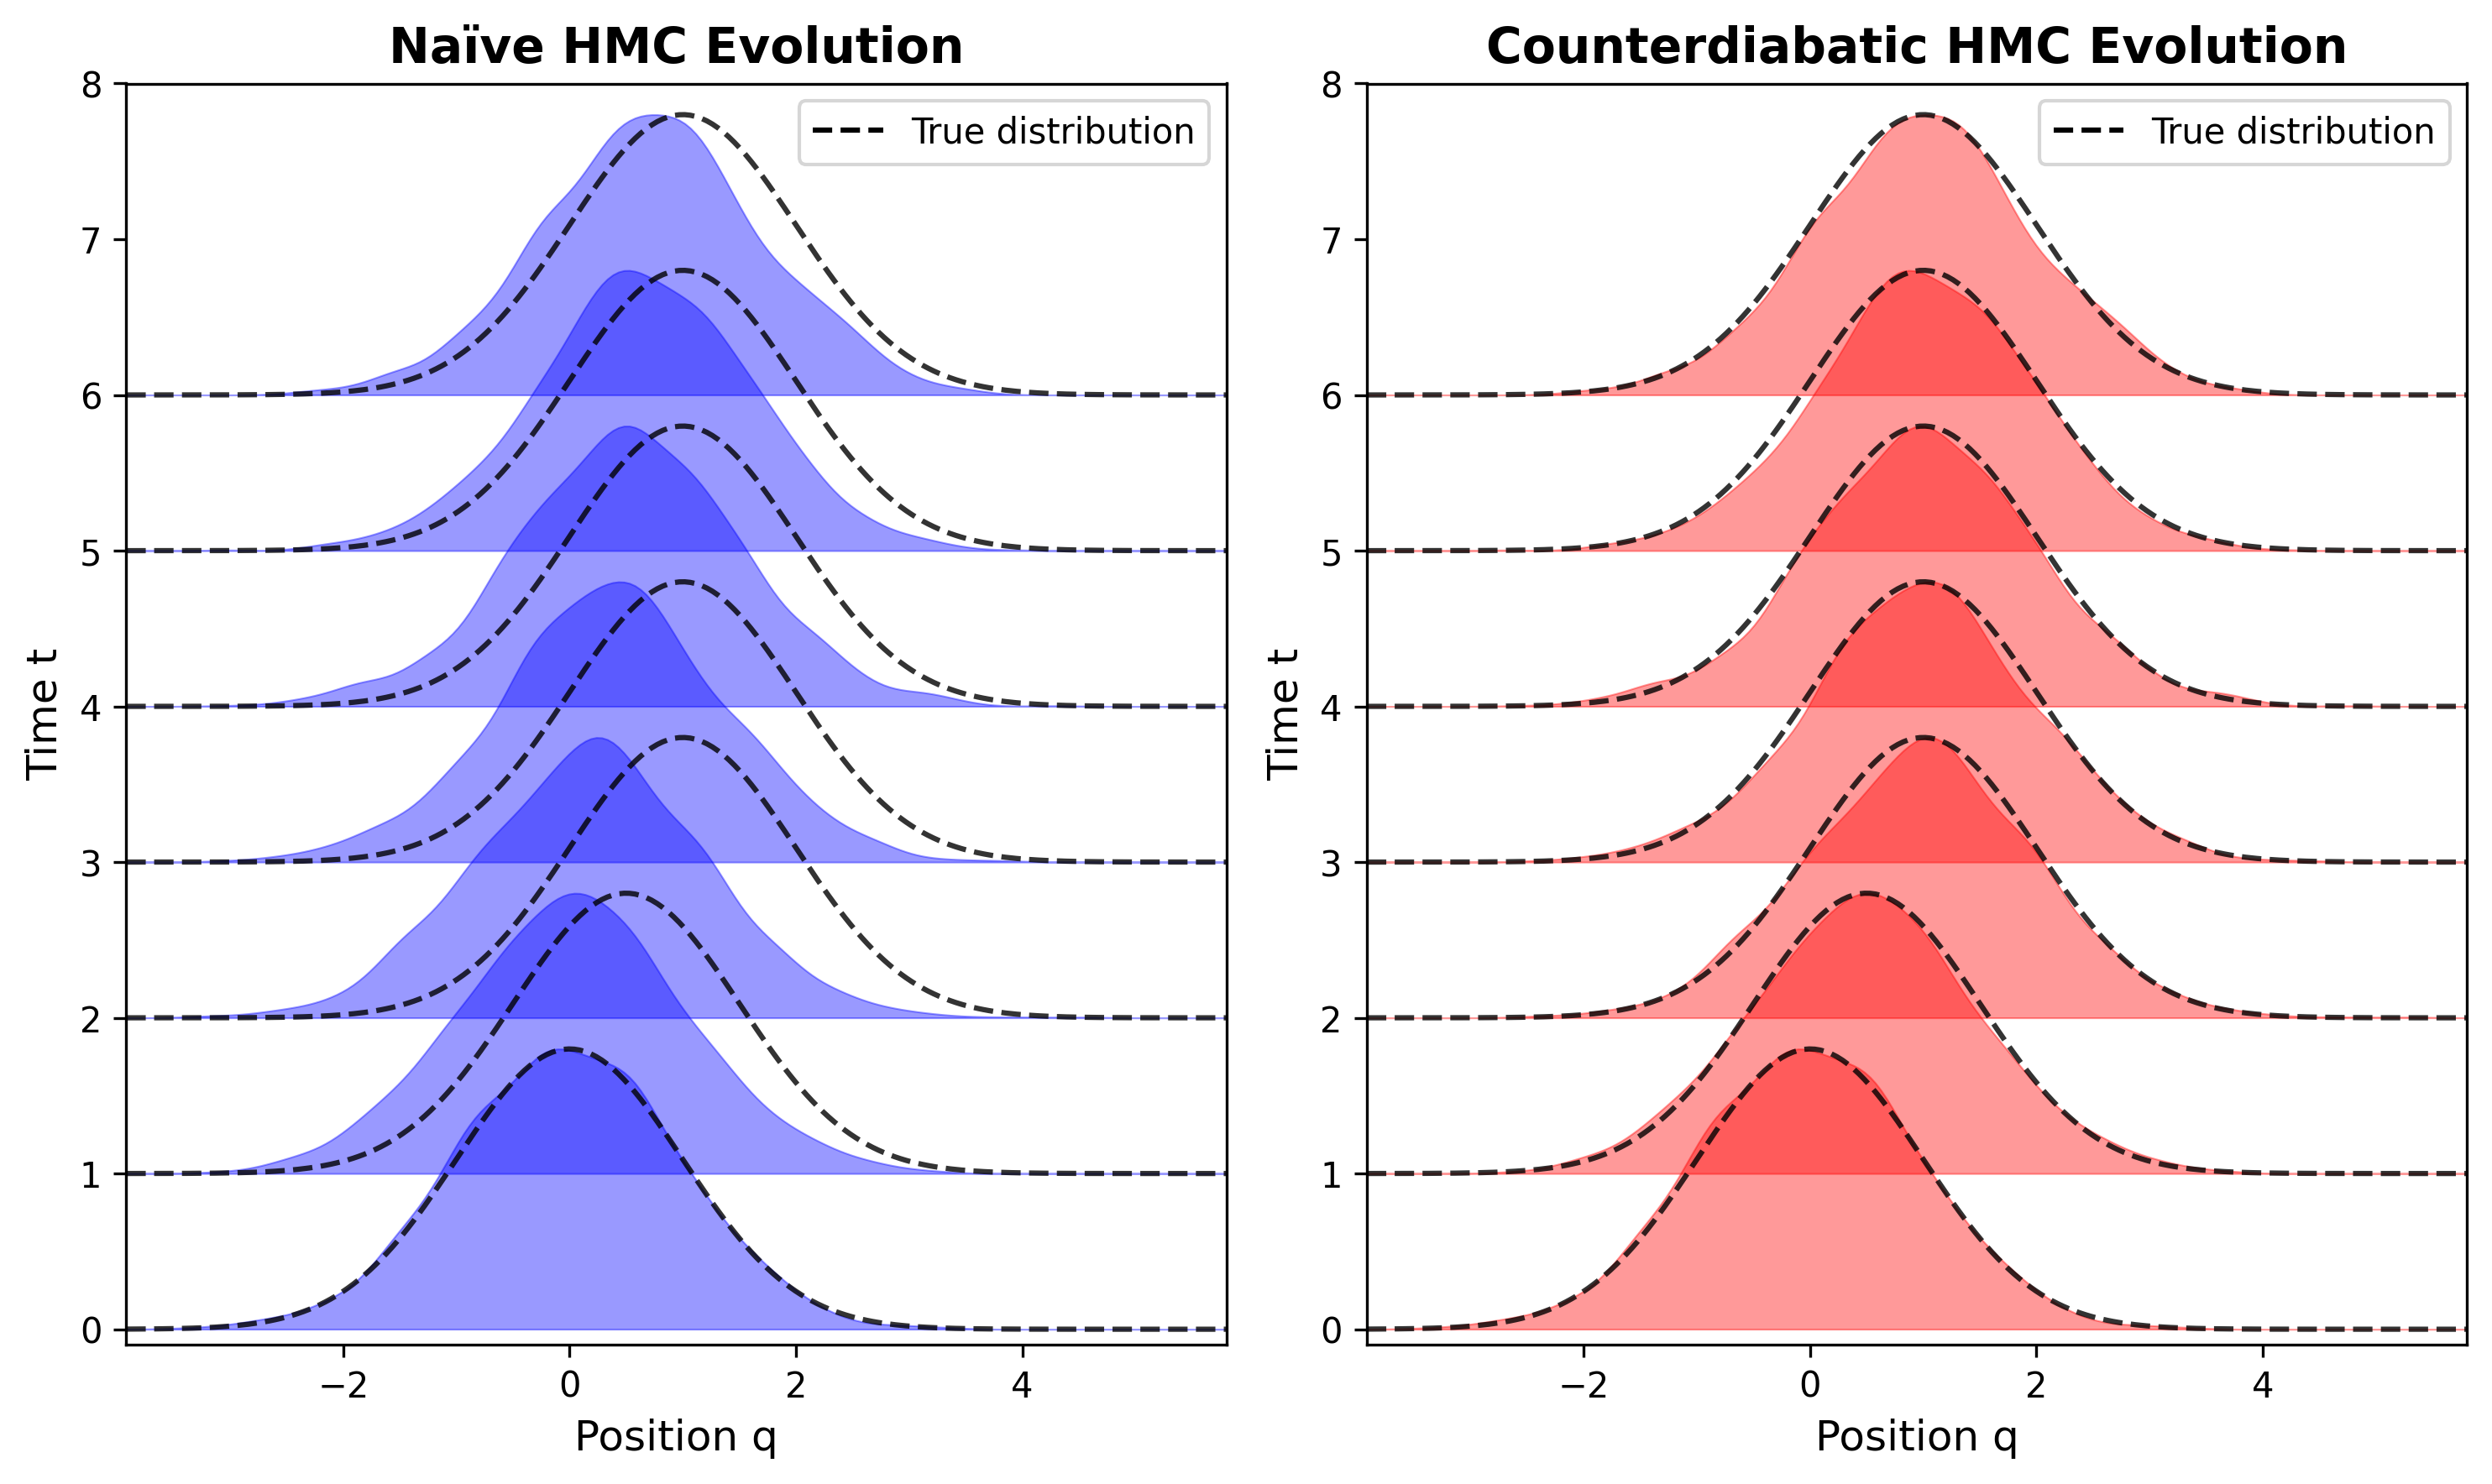
\includegraphics[width=\textwidth]{img/moving_mean_1D.png}
        \caption{A Gaussian with a mean $\lambda(t)$, which moves at constant velocity from $\lambda=0$ to $\lambda=1$, and then remains at $1$. Simply running HMC at each intermediate time step (blue) results in a lag, which is accounted for by the counterdiabatic driving term (red).}
        \label{fig:moving_mean}
    \end{subfigure}
    \hfill
    \begin{subfigure}[b]{0.48\textwidth}
        \centering
        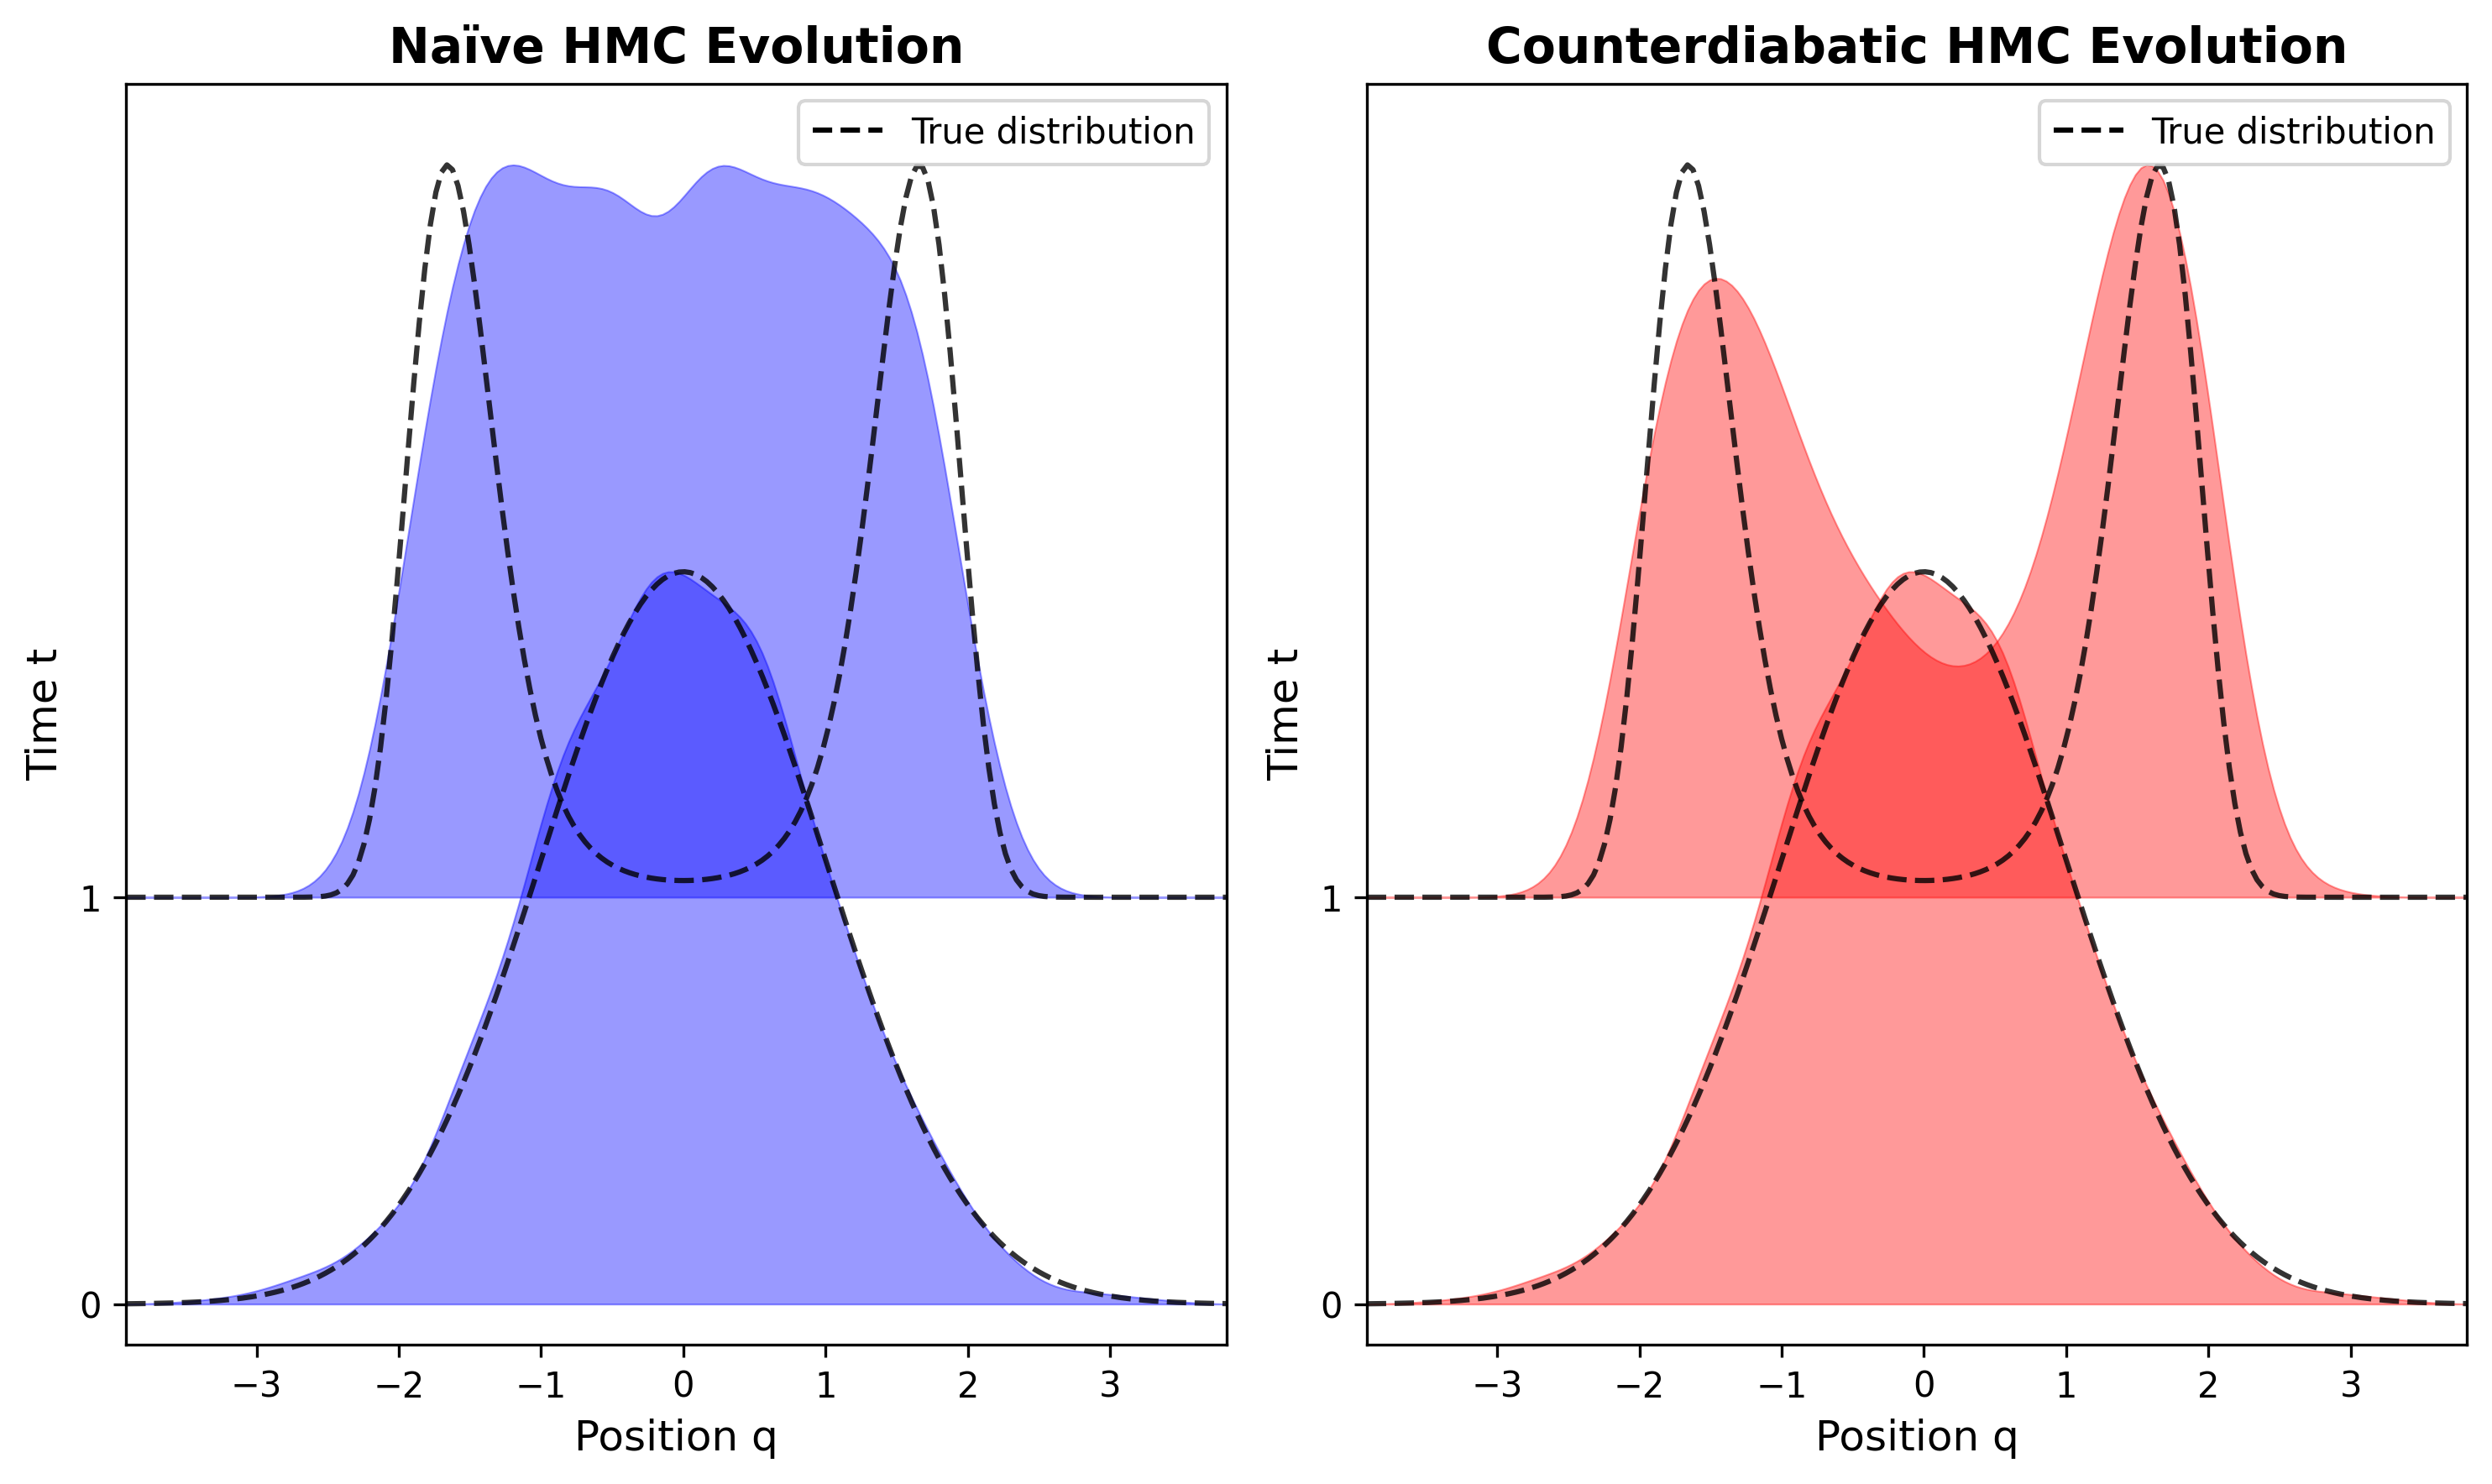
\includegraphics[width=\textwidth]{img/double_well_1D.png}
        \caption{An interpolation between a Gaussian at $t=1$ and a double well at $t=1$. The counterdiabatic driving does not result in a perfect transport, but clearly accelerates the process.}
        \label{fig:double_well}
    \end{subfigure}
    \caption{Illustration of counterdiabatic driving in Hamiltonian Monte Carlo. Left: Moving mean example showing lag and correction. Right: Double well example showing accelerated transport.}
    \label{fig:counterdiabatic_examples}
\end{figure}

In the setting of HMC, moving through a series of distributions in this way corresponds to time evolution of a physical system while changing the system's parameters, a central topic of thermodynamics and statistical mechanics. From this perspective, varying the parameters too quickly results in \emph{lag}, or more physically \emph{dissipation} \cite{vaikuntanathan2011escorted}, where the Hamiltonian flow cannot return to equilibrium quickly enough as the system's parameters change.

% The lag shown in each step corresponds to dissipation or heat transfer \cite{}, while the setting where the jumps between neighbouring distributions are arbitrarily small is known as an \emph{adiabatic} process\footnote{In the language of thermodynamics, \emph{quasistatic} would be the more appropriate term, we use adiabatic in the sense of \cite{sels2017minimizing}}.

Several papers \cite{demirplak2003adiabatic, berry2009transitionless}, both in the quantum and classical setting, have noted that one can compensate for this lag by adding a \emph{counterdiabatic driving term} to the Hamiltonian. More recently, a scheme to approximate this term variationally has been proposed in a quantum setting \cite{sels2017minimizing}. 
We adapt this approach to a classical setting, to obtain a method for transitioning efficiently between a simple tractable distribution and a challenging distribution of interest. We show that our approach is closely related to the proposals of \cite{albergo2024nets, vargas2023transport, arbel2021annealed} among others, but in a Hamiltonian setting.


% Being able to varying a system quickly while staying close to equilibrium (i.e. to the current stationary distribution) is of interest both in classical and quantum physics, and various works \cite{} have proposed adding a driving term to the physical dynamics which allow faster variation of a system's parameters. This is often referred to as \emph{counterdiabatic} driving. 


% This method is best suited to a multi-chain setting, so that instead of a single particle, 

% Crucially, this method is cheap, in the sense that the gradient of the probability density 

% The use of gradient based sampling methods such as Hamiltonian Monte Carlo (HMC), in conjunction with automatic differentiation, has made black box sampling algorithms practical


% In order for MCMC to be statistical efficient, the chain must converge quickly to the target distribution.

% This can be a challenge for many distributions. For example, in a mixture of 2 Gaussians with means that are far apart, an MCMC chain must move through a region of low probability, and if the means are very separately, this may not happen for any feasible simulation length.

% multimodality, since this requires paths to pass through regions of low energy.

% One solution is to define a sequence of distributions, moving from an easy initial distribution to the difficult multimodal target, and at each point in the sequence, run enough steps of MCMC to ensure that the chain (or chains) are stationary for the current distribution. Figure \ref{example} illustrates this approach, in the case 
% TODO: lag...


% In the context of Hamiltonian Monte Carlo, this approach corresponds to varying the Hamiltonian $H(p,q) = TODO$.

% As with HMC generally, physical concepts can here inform statistical algorithm design. Notably, \cite{adiabatic} shows how to vary the Hamiltonian \emph{adiabatically}, i.e. slowly enough that the chain always remains in equilibrium.

% However, adiabatic change is necessarily slow. An avenue of research in many-body quantum physics has investigated adding an additional term to the Hamiltonian to compensate for the lag shown in figure \ref{example}. The details are review in section \cite{todo}, but the approach amounts to adding a term$\ dot\lambda A$ to $H$, where $A$ can be learned in a variational manner.

% While the focus of this technique has been on quantum mechanical systems, the core idea generalizes to classical physics, and indeed, by adding an analogous term $\dot \lambda A$ to the time varying Hamiltonian, where $A$ is estimated at regular intervals, a chain can be made to stay approximately in the current stationary distribution.



% In classical physics, a system is described by a vector $q \in \mathbb{R}^n$ describing a configuration of the system, such as the position of one or more particles, and a second vector $p \in \mathbb{R}^n$. Viewed together, we have a vector $z \in \mathbb{R}^{2n}$ living in the joint position-momentum space (known as phase space). Hamilton's equation of motion (\eqref{ham}) is a first order ODE on this space which determines change of the system over time, which is in turn determined by a function $H(q,p)$ known as the Hamiltonian. The \emph{canonical distribution} $\rho(q,p)\propto e^{-H(q,p)}$ is stationary with respect to the flow induced by $H$.

% Hamiltonian Monte Carlo works by interpreting the space on which an arbitrary distribution with density $\pi$ lives as a physical position space, and chooses a Hamiltonian $H$ in such a way that if $\rho$ is the canonical distribution, then $\pi(q) = \int \rho(q,p)dp$. Since Hamiltonian dynamics can be numerically integrated, this gives rise to a Markov Chain Monte Carlo kernel which approximately 


% Annealing \cite{} and Sequential Monte Carlo (SMC) \cite{} are examples of such approaches. 

\section{Related work}


% Methods which involve moving through a series of  distributions to interpolate from an initial to a final distribution of interest exist at the interface of many fields, including statistics, machine learning, physics and chemistry, and from a variety of perspectives, including optimal transport, stochastic optimal control, molecular dynamics, non-equilibrium physics, and Sequential Monte Carlo. We divide the related work into three main categories.

\paragraph{Sequential Monte Carlo}
In the context of statistics and Bayesian inference, several algorithms exist to deal with the problem of slow convergence to the target distribution. Most relevant to the present work is the application of Sequential Monte Carlo \cite{doucet2001introduction} to sampling from static distributions \cite{del2006sequential}, by constructing a series of distributions with densities $\pi_i$ where $\pi_0$ is the initial distribution and $\pi_T$ is the target distribution. Here a series of particles are evolved according to a Markov kernel targeting the stationary distribution of $\pi_i$ at step $i$, and at each step reweighting and resampling, so that the weighted particles are distributed according to $p_i$.

Several proposals have been made to replace the Markov kernel with one which more effectively transports the particles from $\pi_i$ to $\pi_{i+1}$, including Controlled Sequential Monte Carlo \cite{heng2020controlled} and Schrodinger Bridge SMC \cite{bernton2019schr}.







% Annealed importance sampling \cite{neal2001annealed} draws each successive point $x_i$ in an MCMC chain from a kernel $T_i$, which is stationary for the distribution $\rho(\lambda(i))$. Importance weights \cite{tokdar2010importance} are then used to correct the resulting samples at $x_T$, which depend on the ratio of the initial and final densities. 

% Sequential Monte Carlo \cite{doucet2001introduction} generalizes this approach, by considering a population of $J$ particles $x_i^j$ at each step, which can be resampled with replacement, to prevent all weight falling on a single particle.

% The shortcoming of these methods is that the number of intermediate distributions required for good performance is typically large, and is $O(d^2)$ for the dimensionality of the problem $d$ \cite{todo}. 


\paragraph{Dynamical transport} A separate body of research approaches the problem from the perspective of stochastic optimal control \cite{fleming2012deterministic} and optimal transport \cite{peyre2019computational}. Here, one considers an ODE or SDE governing a variable of interest $x$, which gives rises to a PDE that governs the evolution of the corresponding density $\pi$. The goal is to design the ODE or SDE so that the density $\pi$ evolves from a simple initial distribution to a chosen target distribution.

Among these, Controlled Monte Carlo Diffusions (CMCD \cite{vargas2023transport}), the Liouville Flow Importance Sampler (LFIS \cite{tian2024liouville}), Path Guided Particle Sampling (PGPS \cite{fan2024path}, the Path-Integral Sampler (PIS \cite{zhang2021path}) and Non-equilibrium transport sampling (NETS \cite{albergo2024nets}) all learn a drift term of a differential equation, parametrized by a neural network.
    % Some approaches directly learn a normalizing flow based transport map (Annealed Flow Transport Monte Carlo (AFT) \cite{arbel2021annealed}) or a PDE \cite{sun2024dynamical}, while most consider an ODE or more generally an SDE, whose flow gives rise to this transport map. 

% , in order to correct for lag.

At the intersection of these two perspectives, several recent approaches \cite{albergo2024nets, vargas2023transport} have proposed to use weighting schemes to correct for remaining bias, in the manner of SMC. These are inspired by Jarsynski's equality \cite{jarzynski1997nonequilibrium} and more generally from the detailed fluctuation theorem \cite{crooks1998nonequilibrium}.

\paragraph{Statistical physics} Finally, the problem of transitioning from one stationary distribution to another is a core topic of thermodynamics, and has practical implications for the preparation of physical systems. Adding a term to Hamiltonian dynamics to preserve stationarity through a series of intermediate distributions has been proposed several times in a quantum setting, as \emph{engineered swift equilibration} \cite{martinez2016engineered} and counterdiabatic driving \cite{demirplak2003adiabatic}, where the corresponding problem with a quickly changing Hamiltonian is failure to preserve eigenstates. The core ideas carry over to a classical setting \cite{patra2017shortcuts}, including with stochastic dynamics, often under the name \emph{shortcuts to adiabaticity}, as well as \emph{escorted free energy} (EFE) \cite{vaikuntanathan2011escorted}. We recommend \cite{guery2019shortcuts} for an overview. While the problem is closely related to the optimal transport and control perspectives above, the setting of Hamiltonian dynamics provides useful geometric insights, in particular that the  learned correction to the Hamiltonian can be understood geometrically as a ``gauge potential'', or equivalently as a connection on a fiber bundle \cite{kolodrubetz2017geometry}.
% guery2023driving

The above papers focus on analytic solutions to the driving term for particular physical systems; meanwhile, \cite{sels2017minimizing} proposes \emph{learning} a driving term in a quantum context, but notes that the approach is transferable to a classical setting, which is a central inspiration for our approach.


% goal is to design a transport map from a simple distribution to a more complex, by learning the drift term of a partial differential equation determining the evolution of the density. 



% Several also use weights in order to correct for bias, in particular NETS and CMCD.


% The central difference between these methods and ours is our focus on Hamiltonian Monte Carlo in particular, and therefore on exploiting the special features of Hamiltonian dynamics. While the above methods are concerned with differential equations on the $\mathbb{R}^d$ space on which the target distribution $P$ lives, we consider Hamiltonian dynamics on the phase space of position and momentum, and use the special features of its geometry \cite{} to our advantage. 
% Moreover, we are not learning a drift directly, but rather a term in the Hamiltonian.




% The challenge is then to learn the terms of the differential equation, such as the drift, either in a training phase, or during the sampling procedure.





% In addition, fluctuation theorems from nonequilibrium statistical physics such as Crooks' theorem \cite{} and Jarzynski's equality \cite{} play a key role in schemes to calculate the change in the normalizing constant of the distribution (known in physics as the free energy), which are of use in weighting schemes, as in SMC, and are discussed in \cite{vaikuntanathan2011escorted} and \cite{zhong2024time} as well as in a machine learning context in \cite{vargas2023transport, vaikuntanathan2011escorted, albergo2024nets}.


% One notable approach in this area is Escorted Free Energy (EFE) \cite{vaikuntanathan2011escorted}, which is primarly concerned with learning the free energy (normalization constant) of the final distribution, and does so by adding a term $\dot\lambda u$ to Hamiltonian dynamics, which amounts to the gauge potential we propose. 

% Learning of this term is not considered, which is essential for our goal of applying this method to arbitrary distributions with differentiable densities, but see \cite{asymmetric} for a method to learn the driving term based on entire backward and forward trajectories. Similar remarks apply to \cite{demirplak2003adiabatic}, which is one of the early papers to propose a counterdiabatic driving term, but only considers analytic methods to obtain it. More generally, the focus in much of the work here \cite{patra2017shortcuts} is on analytic solutions to the driving term for special cases.

\paragraph{Contributions} Since Hamiltonian Monte Carlo is the gold standard approach for sampling from differentiable densities, it is natural that schemes for accelerating convergence to stationarity should focus on it. We emphasize this focus as the main ingredient by which our method differs from the recent approaches to sampling with learning discussed above.

% our focus on Hamiltonian Monte Carlo, and the simplicity of the learning problem, which requires only the gradient of the log density, which has already been calculated in the course of performing standard HMC steps, as we outline in section \ref{sec:todo}.

Table \ref{table1} summarizes what we consider to be the most similar approaches to our own and the relevant differences. All of the listed methods take a population of particles, and evolve them, while also varying the distribution from an easy initial distribution to a target of interest. \emph{Dynamics} refers to the way in which particles are updated at each step, \emph{Weights} to whether a weighting scheme is used to correct the distribution of particles, \emph{Learned term} to what, if any, term needs to be learned for the dynamics, and \emph{Amortized} to whether the algorithm requires a phase before runtime in which training takes place (as opposed to any training happening during the evolution of the particles).


% Several methods have been proposed, in the context of sampling, to learn a transport map to counteract lag induced by a changing distribution. Meanwhile, in the context of quantum physical systems, methods have been proposed to learn a driving term $A$ in a Hamiltonian to correct an analogous ``dissipation''.

% However, to our knowledge, no previous work has proposed learning $A$ in the context of sampling. Since Hamiltonian Monte Carlo is the gold standard approach for sampling from differentiable densities, this is a natural approach, and one which we pursue in the rest of the paper. We envision it as the right way to overcome slow burn-in for any differentiable sampling problems where this is a problem.






% Most closely related to the present work are approaches which evolve a particle or particles according to a dynamics $x(t)$ given by an SDE, so that by the Fokker-Planck formula:

% \nabla\cdot (b_t\rho_t)


 
% \cite{sun2024dynamical}: pde to transport the measure

% \cite{arbel2021annealed} 
% ``An alternative approach is to build a transport map T :
% X → X to ensure that if X ∼ π0 then the distribution
% of X0 = T(X) denoted T#π0 is approximately equal to
% π. '': this paper trains a normalizing flow to transport from one distribution to the next.

% In the context of computational physics and chemistry, \cite{vaikuntanathan2011escorted} propose a 
% `` The dissipation is positive as a consequence of the second law of thermodynamics, and reflects the lag that builds up as the system pursues – but is unable to keep pace with – the equilibrium distribution corresponding to the continuously changing parameter λ''
% ``The approach we take here is motivated by previous work [12–
% 15] and involves generating artificial, or “escorted”, trajectories, Eq. 10, by modifying the dynamics
% with terms that directly couple the evolution of the system to changes in the external parameter.''

% dries
% berry2009transitionless


\begin{center}
\begin{tabular}{||c c c c c c||} 
\label{table1}
 Method & Dynamics & Weights & Learned term & Amortized & Field \\ [0.5ex] 
 \hline
 CSMC & Markov kernel & Yes & Kernel & Yes & Stats \\ 
 EFE \cite{vaikuntanathan2011escorted} & Hamiltonian & No & None & No & Phys/Chem  \\ 
 APTCF \cite{demirplak2003adiabatic} & Hamiltonian & No & None & No & Chem  \\ 
 AIS \cite{neal2001annealed} & MCMC & Yes & None & No & Stats \\
 NETS \cite{albergo2024nets} & Overdamped Langevin & Yes & Drift & Yes & ML  \\ 
 CMCD \cite{vargas2023transport}  & Langevin & No (?) & Drift & Yes & ML  \\ 
 AFT \cite{arbel2021annealed} & NF + MCMC & Yes & NF Map & No & ML \\ 
 LFIS \cite{tian2024liouville} & ODE & No & Drift & No & ML  \\ 
 PGPS \cite{fan2024path} & ODE & No & Drift & No & ML \\ 
 DMT \cite{sun2024dynamical} & PDE & No & Drift & No & ML/PDEs \\ 
 PIS \cite{zhang2021path} & SDE & Yes & Drift & Yes & ML/Control  \\ 
  % & & & & &  \\ 
 CMC (ours) & Hamiltonian & No & Gauge field & No & ML/Phys \\ 
\end{tabular}
\end{center}

% FEAT paper is the most useful one...

% todo: nets tries also learning $\phi$, the potential function...

% crooks paper: https://arxiv.org/pdf/1105.2278

% todo: include Path-Guided Particle-based Sampling

% todo: minimal work protocols, e.g. Beyond Linear Response: Equivalence between Thermodynamic Geometry and Optimal Transport: applied maths: a relationship between counterdiabatic stuff (in overdamped setting) and optimal control, via geometry

% A dynamical systems framework for intermittent data assimilation

% todo: engineered swift equilibration

% Time-Asymmetric Fluctuation Theorem: see this paper...

% Control, Transport and Sampling: Towards Better Loss Design

% weights: crooks paper on discretization work proposed weighting by the exponential of the work

% Neural Adaptive Sequential Monte Carlo


\section{Counterdiabatic Monte Carlo}

\paragraph{Hamiltonian dynamics}

Suppose we have a physical system given by a $d$ dimensional vector $q \in \mathbb{R}^d$ $d$, such as the position of a particle. Hamilton's equations of motion are a 1st order ODE defined on $(q,p) \in \mathbb{R}^{2d}$, where $p$ is a second variable called the momentum. The ODE is defined in terms of a real-valued \emph{Hamiltonian} function $H(q,p)$.

\begin{align}
\dot{q} &= \nabla_p H(q,p) \\
\dot{p} &= -\nabla_q H(q,p)
\end{align}

We refer to the solution to the ODE as the \emph{flow} $\phi_H$, so that $\phi_H(q_0,p_0,t)$ is the state of the system at time $t$ given the initial state $(q_0,p_0)$.


\paragraph{Poisson bracket} If $f$ is also a real valued function of $(q,p)$, then the time derivative $\partial_tf$ can be written as the \emph{Poisson bracket} $\partial_tf(q,p) = \{f, H\}(q,p) := \nabla_q f \cdot \nabla_p H - \nabla_p f \cdot \nabla_q H$.

We note that the Poisson bracket is antisymmetric, i.e. $\{A, B\} = -\{B, A\}$, and that $\int C(q,p) \{A, B\}(q,p) dqdp = \int B(q,p) \{C, A\}(q,p) dqdp$.

\paragraph{Canonical distribution} The \emph{canonical distribution} defined as $\rho_H(q,p) \propto e^{-H(q,p)}$ is a stationary distribution of Hamiltonian dynamics. Indeed, the continuity equation $\partial_t\rho_H = \{H, \rho_H\}$ implies that $\partial_t\rho_H = 0$, by an above property of the Poisson bracket. We denote by $\phi^*_H$ the flow of the differential equation, so that $\phi^*_H(t')(\rho_H) = \rho_H$.

% \paragraph{The continuity equation} The continuity equation is a partial differential equation which describes the time evolution of the probability density function of a particle subject to Brownian motion. It is given by:

% $$
% \partial_t\rho = -\nabla \cdot (\rho) = \{H, \rho\}
% $$

% where $b$ is the drift term and $\sigma$ is the diffusion term.

\paragraph{Hamiltonian Monte Carlo} The principle of Hamiltonian Monte Carlo is to use a discretization of Hamiltonian dynamics to produce a kernel which has a stationary distribution $\rho_H$ for which the marginal on $q$, i.e. $\pi(q) \propto \int \rho_H(q,p) dp$, is the distribution of interest. This can be achieved by choosing $H = -\nabla\log\pi(q) + \frac{1}{2}|p|^2$, which only requires knowing the density up to the normalization constant.

The Metropolis-Hastings algorithm \cite{chib1995understanding} is used to correct for bias coming from the discretization of the Hamiltonian dynamics, and momentum can be refreshed every $n$ steps, or partially refreshed every step, in order to ensure ergodicity.


\subsection{Counterdiabatic driving}
% One solution is to have a time varying $H$, where $\rho_{H(\lambda(0))}$ is a distribution that is easy to sample from, and $\rho_{H(\lambda(T))}$ is the distribution of interest. What we want is an ODE which gives $\partial_t\rho_{H(\lambda(t))}=0$, so that $\phi_{H(\lambda(t))}^*(t')\rho_{H(\lambda(t))} = \rho_{H(t+t')}$

When $H$ is time dependent, for example through a parameter $\lambda$, we can consider the time dependent flow $\phi_{H(\lambda(t))}$. Crucially, we note that $\partial_t\rho_{H(\lambda(t))} \neq 0$, so that $\phi^*_{H}(t')\rho_{H(\lambda(t))} \neq \rho_{H(\lambda(t+t'))}$. In other words, the flow of the time-varying Hamiltonian does not preserve the time-varying distribution $\rho_{H(\lambda(t))}$. If it did, we could simply run Hamiltonian dynamics with $H(\lambda(t))$ and obtain at time $T$ the intended target perfectly. To see why it fails, we proceed as follows:

% But the naive approach, which is to follow the now time-dependent Hamiltonian dynamics, i.e. $\dot z(t) = \Omega \frac{\partial H(z,t)}{\partial z}$, does not work, in the sense that $\partial_tH$ is not $0$, which means that the stationary distribution at each time $t$ is not $\rho_{H(t)}$. To see this:


$$
\partial_t\rho_{H(\lambda(t))} = \{H, \rho_{H(\lambda(t))}\} + \dot\lambda\partial_\lambda \rho_{H(\lambda(t))}
$$

$$
= 0 - \dot\lambda\partial_\lambda H\rho_{H(\lambda(t))} - \dot\lambda\frac{\partial \log Z}{\partial \lambda}\rho_{H(\lambda(t))} = (-\partial_\lambda H + \langle \partial_\lambda H\rangle_t) \dot\lambda\rho_{H(\lambda(t))}
$$



% One way to deal with this discrepancy is to make $\partial_\lambda H$ small, by changing time very slowly. In physical terms, this corresponds to adiabatic change of $H$. \cite{} shows how to vary $\lambda$ adiabatically), but for difficult distributions, this will naturally be slow. Another option is to take many steps of the kernel at each value of $t$, to re-equilibrate. This suffers from essentially the original problem: potentially slow thermalization.

\cite{demirplak2003adiabatic}, \cite{berry2009transitionless} and \cite{vaikuntanathan2011escorted, guery2023driving} note\footnote{Here, the focus is on quantum systems, but by the correspondence between Poisson brackets and commutators, the central insight may be translated to a classical setting, as explained in \cite{}.} that one can offset the lag by introducing a term $A$, known as the \emph{counterdiabatic gauge potential}, with the property that $\{A, H\} = \partial_\lambda H - \langle \partial_\lambda H\rangle_t$. Then we would have:

$$
\partial_\lambda\rho_{H(\lambda(t))} = \{H, A\}\rho_{H(\lambda(t))} = \{\rho_{H(\lambda(t))}, -A\} = \{A, \rho_{H(\lambda(t))}\} 
$$

This can be interpreted as the evolution of the distribution that would be generated by a Hamiltonian $A$. This demonstrates a remarkable result: if we choose as our Hamiltonian $H + \dot\lambda$, we have that $\phi^*_{H+\dot\lambda A}(t')\rho_{H(\lambda(t))} = \rho_{H(\lambda(t+t'))}$.

% that we can directly set our Hamiltonian to $H_{CD} = H + \dot\lambda A$, so as to match the distributional change arising from the time varying Hamiltonian.


\paragraph{Learning the counterdiabatic gauge potential}

\cite{sels2017minimizing} demonstrates that one can variationally approximate $A$ in a computationally practical way. In classical terms, the key idea is that we minimize $\mathbb{E}_{z \sim \rho_{H(\lambda(t))}}[|G(z)|^2]$ at each time point $t$, where 

$$
G(z) = \{A, H\}(z) - \partial_\lambda H(z) + \mathbb{E}[ \partial_\lambda H(z)]
$$

Multiplying out, we find $\mathbb{E}[|G(z)|^2] = \mathbb{E}[\{A, H\}^2 + (\partial_\lambda H)^2 + \mathbb{E}[\partial_\lambda H]^2 - 2\{A, H\}(\partial_\lambda H) + 2\{A, H\}\mathbb{E}[\partial_\lambda H] - 2(\partial_\lambda H)\mathbb{E}[\partial_\lambda H]] = \mathbb{E}[\{A, H\}^2 + (\partial_\lambda H)^2 - 2\{A, H\}(\partial_\lambda H) + 2\{A, H\}\mathbb{E}[\partial_\lambda H] - \mathbb{E}[ \partial_\lambda H]^2] $ 

But we can see that a minimum of the following:

$R(z) = \langle |\{A(z), H(z)\} - \partial_\lambda H(z)|^2 \rangle = \langle \{A(z), H(z)\}^2 -2\{A(z), H(z)\}\partial_\lambda H(z) + (\partial_\lambda H(z))^2 \rangle$

is a minimum of $|G|^2$, since when $\partial_\lambda H = \{A, H\}$, we find that $\langle \partial_\lambda H \rangle = \langle \{A, H\}\rangle = \int \rho \{A, H\} dz  = \int A \{\rho, H\} = 0$, where the penultimate step follows by an above property of the Poisson bracket.

% the final two terms disappear by the same arguments as above when $\partial_\lambda H = \{A, H\}$.
This means that we can minimize $\mathbb{E}[R(A, H)] = \mathbb{E}[|\{A, H\} - \partial_\lambda H|^2 ]\rangle$ instead, which is simple to calculate.






% \subsection{Hamiltonian Monte Carlo}

% Let $\rho_H$ be the canonical distribution, i.e. $\rho_H(q,p) \propto e^{-H(q,p)}$. Exact Hamiltonian flow under a given $H$ preserves $\rho_H$. That is, $\partial_t\rho_H = \{H, \rho_H\} = 0$ and $\phi_H^*(t')\rho_H = \rho_H$, where $\phi$ is the flow of the differential equation. 

% In practice, Hamiltonian Monte Carlo uses discretized Hamiltonian dynamics as a kernel, and accounts for the bias induced by discretization by the Metropolis-Hastings algorithm \cite{}. To ensure ergodicity, momentum can be refreshed every $n$ steps, or partially refreshed every step, which corresponds to the discretization of underdamped Langevin dynamics \cite{}. 

% When running HMC, one initializes by drawing an initial sample $q$ (or population of samples $q_i$) from a simple distribution, such as a Gaussian, and the momentum $p$ similarly, to obtain a state $z=(q,p)$. As one evolves $z$ according to the kernel, the distribution it follows evolves towards $\rho_H$. This phase of the algorithm is known in the language of statistical physics as thermalization, i.e. the process of the ensemble evolving to thermal equilibrium. Typically, one only wants to collect samples after this phase, so one discards early samples, a procedure known as burn-in. Furthermore, early steps of the algorithm may be used to choose hyperparameters, such as the discretization step size.

% In some problems, the thermalization phase is straightforward, and the bottleneck is the efficiency of the next phase, where the number of effectively independent samples is determined by the autocorrelation of the kernel. However, in this paper we are concerned with problems where thermalization is difficult. A motivating example is a mixture of two 1D Gaussians, which in physical terms corresponds to a double well potential. If the means on the two Gaussians are separated by a large distance, the position according to Hamiltonian dynamics will struggle to move between the wells, because it requires moving through an energetically unfavourable region. As such, thermalization could take extremely long, even if it is guaranteed in the limit of infinite time.


\subsection{Weighting}

When performing the algorithm described above, bias, in the sense of the population of particles at time $t$ failing to agree with $\rho_{H(t)}$ arises from two sources. The first is the numerical discretization of Hamilton's equations of motion. The second is the fact that we only approximate the true counterdiabatic driving term $A$.
% 

Bias in of itself is not a problem; once we have approached close to the final stationary distribution, HMC with Metropolis adjustment can be used to remove remaining bias. However, since the learning of $A$ requires high quality samples from each successive distribution, bias removal is important.


and emphasize that we resample using the weights along the path of distributions, rather than only using the weights 
    This is important, since the weighted particles are used to calculate the expectation required for the learning of $A$.
    We note that this is an important difference (CHECK) to NETS.

Here, we follow SMC:

that the weight is determined by a ratio (or more technically the Radon-Nikodym derivative) of the form:

$$
\frac{d(L_{t-1}\otimes \gamma_t)}{d( \gamma_{t-1} \otimes M_t)}(z_{t-1},z_t)
$$

In the simplest case, $M$ can be chosen as any invariant kernel, and $L$ as its time reversal, i.e. $L_{t-1}(z_t, z_{t-1})\pi_{t}(z_t) = \pi_t{z_{t-1}}M_t(z_{t-1}, z_t)$.

In many cases, the ratio of kernels derived from forward and backward dynamics is known as a result of the Crooks detailed fluctuation theorem \cite{crooks1998nonequilibrium}. This states that

$$

$$







Weighting schemes can remove bias, and \cite{zhong2024time} gives the general form of the weight in the presence of a counterdiabatic driving term.

$$dW = \frac{\partial H}{\partial t} - \nabla H\cdot \nabla A + \nabla^2 A$$

which defines $W[z(t)] = \int_0^T dW$

This allows us to calculate the reversibility, since \cite{zhong2024time} show that 

W[z(t)] = H(z(t), \lambda(t)) - H(z(0), \lambda(0)) + \log \frac{\mathcal{P}[z(t) | z(0)}{\mathcal{P}(\tilde z(t) | \tilde z(0)}


% (We see that if we were to stay (via canonical transformation) in the frame of the moving Hamiltonian, i.e. by taking the total derivative, we would experience an effective Hamiltonian $-A$.)

% But then we need only use a Hamiltonian $H - \dot\lambda A$ to arrive at $\partial_t\rho_{H(\lambda(t))} = 0$.


\section{Algorithm design}

The fact that we can learn an approximation of $A$ suggests an algorithm for sampling. We first choose a path of densities $\pi(q;\lambda(t))$ where $\pi(q;\lambda(0))$ is chosen to be straightforward to sample from, and where $\pi(q;\lambda(T))$ is the distribution of interest. This defines a time varying Hamiltonian $H(p,q; \lambda(t)) = - \nabla \log \pi(q;\lambda(t)) + \frac{1}{2}|p|^2$. 

We then initialize a population of particles in $\pi(\cdot ; \lambda(0))$, distributed according to $\rho_{H(\lambda(0))}$. At each time $t$, discretized in steps of length $\epsilon$, we minimize the \emph{expectation} of $R$, under the empirical distribution of the current population, to obtain an estimate of $A$ (Algorithm \ref{alg:fit-agp}). We use $H(\cdot ; \lambda(t)) + \dot\lambda A(\cdot ; \lambda(t))$ as our Hamiltonian at a given time $t$. Further, we have the option of computing weights according to \eqref{todo} after each time step, which correct for the bias introduced by the numerical discretization of the dynamics and the approximation of $A$. This is summarized in Algorithm \ref{alg:cd-hmc}.

This can be understood as a special case of the general framework of Sequential Monte Carlo samplers \cite{doucet2001sequential}, as shown in appendix TODO.

\paragraph{Numerical Integration} A key complication is that $A$ is not separatable into a term depending on $p$ and a term depending on $q$. This means that the Velocity Verlet integrator is not symplectic.




% We present our algorithm in the framework of Sequential Monte Carlo samplers \cite{doucet2001sequential}.

% In your preamble:
% \usepackage{algorithm}
% \usepackage{algpseudocode}
% \usepackage{amsmath, amssymb}

% Notation:
% Target density \pi(q) \propto \exp[-U(q;\lambda=1)] with unit mass matrix.
% Hamiltonian along protocol: H_\lambda(q,p) = U(q;\lambda) + \tfrac12 |p|^2.
% Counterdiabatic Hamiltonian: H^{\text{CD}}(q,p,t) = H_{\lambda(t)}(q,p) + \dot{\lambda}(t)\,A_\phi(q,p;\lambda(t)).
% Poisson bracket: \{A,H\} = \nabla_q A \cdot p - \nabla_q U(q;\lambda) \cdot \nabla_p A.

\begin{algorithm}[t]
    \caption{Fit adiabatic gauge potential $A_\phi$ at a given $\lambda$}
    \label{alg:fit-agp}
    \begin{algorithmic}[1]
    \Require Real-valued function $A_\phi(q,p;\lambda)$, optimizer (e.g. Adam)\;, schedule $\lambda_i$, population of particles $\{q_i,p_i\}_{i=1}^N$, number of iterations $T$.
    \For{$t=1,\dots,T$}
    %   \State Sample $q \sim \pi_\lambda(q) \propto e^{-U(q;\lambda)}$\; and $p \sim \mathcal{N}(0,I)$
    % = \mathbb{E}[r^2(q,p,\lambda;\phi)]
      \State Compute $l  \gets \frac{1}{N}\sum_{i=1}^N \{A_\phi,H_\lambda\}(q_i,p_i) - \partial_\lambda U(q_i;\lambda)$
      \State Update $\phi$ using optimizer with loss $l$
    \EndFor
    \State \Return $\phi$
    \end{algorithmic}
    \end{algorithm}
    
    \begin{algorithm}[t]
    \caption{Counterdiabatic HMC (CHMC) with population and weighting}
    \label{alg:cd-hmc}
    \begin{algorithmic}[1]
    \Require Population $\{q_i^{(0)}\}_{i=1}^N$ from initial distribution\;; potential $U(q;\lambda)$ and gradients\;; step size $\varepsilon$\;; schedule $\{\lambda_k\}_{k=1}^L$ with $\lambda_1=0$ (easy) and $\lambda_L=1$ (target)\;; learned $A_\phi(q,p;\lambda)$ and its partials $\nabla_q A_\phi,\nabla_p A_\phi$.
    \State Initialize weights $w_i^{(0)} = 1/N$ for all $i$
    \For{$k=1$ to $L-1$}
      \For{$i=1$ to $N$}
        \State Sample $p_i \sim \mathcal{N}(0,I)$
        \State Set $(q,p) \leftarrow (q_i^{(k-1)}, p_i)$; set $W_i \leftarrow 0$
        \State \textbf{Half-kick} (potential \& CD-$q$ force): 
        \[
          p \leftarrow p - \tfrac{\varepsilon}{2}\Big(\nabla_q U(q;\lambda_k) + \dot{\lambda}_k \,\nabla_q A_\phi(q,p;\lambda_k)\Big)
        \]
        \State \textbf{Drift} (kinetic \& CD-$p$ flow):
        \[
          q \leftarrow q + \varepsilon\Big(p + \dot{\lambda}_k\, \nabla_p A_\phi(q,p;\lambda_k)\Big)
        \]
        \State \textbf{Protocol work increment} (discrete $\partial_t H^{\text{CD}}$):
        \[
          W_i \leftarrow W_i + \Big(U(q;\lambda_{k+1}) - U(q;\lambda_k)\Big) 
          + \Big(\dot{\lambda}_{k+1}A_\phi(q,p;\lambda_{k+1}) - \dot{\lambda}_k A_\phi(q,p;\lambda_k)\Big)
        \]
        \State \textbf{Half-kick} (with updated waypoint):
        \[
          p \leftarrow p - \tfrac{\varepsilon}{2}\Big(\nabla_q U(q;\lambda_{k+1}) + \dot{\lambda}_{k+1}\,\nabla_q A_\phi(q,p;\lambda_{k+1})\Big)
        \]
        \State Update particle: $q_i^{(k)} \leftarrow q$
        \State Update weight: $w_i^{(k)} \leftarrow w_i^{(k-1)} \exp(-W_i)$
      \EndFor
      \State Normalize weights: $w_i^{(k)} \leftarrow w_i^{(k)} / \sum_j w_j^{(k)}$
      \State Optionally resample if effective sample size is low
    \EndFor
    \State \Return weighted population $\{(q_i^{(L)}, w_i^{(L)})\}_{i=1}^N$
    \end{algorithmic}
    \end{algorithm}

\paragraph{Choice of step size} As in standard HMC, the choice of $\epsilon$ is a trade-off between the accuracy of the dynamics and the efficiency of the algorithm. We propose to tune step size by monitoring the error in $H$; in the limit of small step size and perfect $A$, $H$ should be preserved exactly. 

consider fisher score

\section{Evaluation}

The goal of CHMC is to reduce the wall-clock time required to sample from challenging distributions. We consider the regime where the gradient of the log density is costly, so that our central focus is on the number of calls to this gradient function required for an \emph{effective sample size} of 100 samples.

We compare to Sequential Monte Carlo, as well as the results reported in NETS TODO 

We use the models proposed in the NETS paper for evaluation (todo: get michael or eric to share them).

\section{Conclusion}

\newpage
\section*{NeurIPS Paper Checklist}

%%% BEGIN INSTRUCTIONS %%%
The checklist is designed to encourage best practices for responsible machine learning research, addressing issues of reproducibility, transparency, research ethics, and societal impact. Do not remove the checklist: {\bf The papers not including the checklist will be desk rejected.} The checklist should follow the references and follow the (optional) supplemental material.  The checklist does NOT count towards the page
limit. 

Please read the checklist guidelines carefully for information on how to answer these questions. For each question in the checklist:
\begin{itemize}
    \item You should answer \answerYes{}, \answerNo{}, or \answerNA{}.
    \item \answerNA{} means either that the question is Not Applicable for that particular paper or the relevant information is Not Available.
    \item Please provide a short (1–2 sentence) justification right after your answer (even for NA). 
   % \item {\bf The papers not including the checklist will be desk rejected.}
\end{itemize}

{\bf The checklist answers are an integral part of your paper submission.} They are visible to the reviewers, area chairs, senior area chairs, and ethics reviewers. You will be asked to also include it (after eventual revisions) with the final version of your paper, and its final version will be published with the paper.

The reviewers of your paper will be asked to use the checklist as one of the factors in their evaluation. While "\answerYes{}" is generally preferable to "\answerNo{}", it is perfectly acceptable to answer "\answerNo{}" provided a proper justification is given (e.g., "error bars are not reported because it would be too computationally expensive" or "we were unable to find the license for the dataset we used"). In general, answering "\answerNo{}" or "\answerNA{}" is not grounds for rejection. While the questions are phrased in a binary way, we acknowledge that the true answer is often more nuanced, so please just use your best judgment and write a justification to elaborate. All supporting evidence can appear either in the main paper or the supplemental material, provided in appendix. If you answer \answerYes{} to a question, in the justification please point to the section(s) where related material for the question can be found.

IMPORTANT, please:
\begin{itemize}
    \item {\bf Delete this instruction block, but keep the section heading ``NeurIPS Paper Checklist"},
    \item  {\bf Keep the checklist subsection headings, questions/answers and guidelines below.}
    \item {\bf Do not modify the questions and only use the provided macros for your answers}.
\end{itemize} 
 

%%% END INSTRUCTIONS %%%


\begin{enumerate}

\item {\bf Claims}
    \item[] Question: Do the main claims made in the abstract and introduction accurately reflect the paper's contributions and scope?
    \item[] Answer: \answerTODO{} % Replace by \answerYes{}, \answerNo{}, or \answerNA{}.
    \item[] Justification: \justificationTODO{}
    \item[] Guidelines:
    \begin{itemize}
        \item The answer NA means that the abstract and introduction do not include the claims made in the paper.
        \item The abstract and/or introduction should clearly state the claims made, including the contributions made in the paper and important assumptions and limitations. A No or NA answer to this question will not be perceived well by the reviewers. 
        \item The claims made should match theoretical and experimental results, and reflect how much the results can be expected to generalize to other settings. 
        \item It is fine to include aspirational goals as motivation as long as it is clear that these goals are not attained by the paper. 
    \end{itemize}

\item {\bf Limitations}
    \item[] Question: Does the paper discuss the limitations of the work performed by the authors?
    \item[] Answer: \answerTODO{} % Replace by \answerYes{}, \answerNo{}, or \answerNA{}.
    \item[] Justification: \justificationTODO{}
    \item[] Guidelines:
    \begin{itemize}
        \item The answer NA means that the paper has no limitation while the answer No means that the paper has limitations, but those are not discussed in the paper. 
        \item The authors are encouraged to create a separate "Limitations" section in their paper.
        \item The paper should point out any strong assumptions and how robust the results are to violations of these assumptions (e.g., independence assumptions, noiseless settings, model well-specification, asymptotic approximations only holding locally). The authors should reflect on how these assumptions might be violated in practice and what the implications would be.
        \item The authors should reflect on the scope of the claims made, e.g., if the approach was only tested on a few datasets or with a few runs. In general, empirical results often depend on implicit assumptions, which should be articulated.
        \item The authors should reflect on the factors that influence the performance of the approach. For example, a facial recognition algorithm may perform poorly when image resolution is low or images are taken in low lighting. Or a speech-to-text system might not be used reliably to provide closed captions for online lectures because it fails to handle technical jargon.
        \item The authors should discuss the computational efficiency of the proposed algorithms and how they scale with dataset size.
        \item If applicable, the authors should discuss possible limitations of their approach to address problems of privacy and fairness.
        \item While the authors might fear that complete honesty about limitations might be used by reviewers as grounds for rejection, a worse outcome might be that reviewers discover limitations that aren't acknowledged in the paper. The authors should use their best judgment and recognize that individual actions in favor of transparency play an important role in developing norms that preserve the integrity of the community. Reviewers will be specifically instructed to not penalize honesty concerning limitations.
    \end{itemize}

\item {\bf Theory assumptions and proofs}
    \item[] Question: For each theoretical result, does the paper provide the full set of assumptions and a complete (and correct) proof?
    \item[] Answer: \answerTODO{} % Replace by \answerYes{}, \answerNo{}, or \answerNA{}.
    \item[] Justification: \justificationTODO{}
    \item[] Guidelines:
    \begin{itemize}
        \item The answer NA means that the paper does not include theoretical results. 
        \item All the theorems, formulas, and proofs in the paper should be numbered and cross-referenced.
        \item All assumptions should be clearly stated or referenced in the statement of any theorems.
        \item The proofs can either appear in the main paper or the supplemental material, but if they appear in the supplemental material, the authors are encouraged to provide a short proof sketch to provide intuition. 
        \item Inversely, any informal proof provided in the core of the paper should be complemented by formal proofs provided in appendix or supplemental material.
        \item Theorems and Lemmas that the proof relies upon should be properly referenced. 
    \end{itemize}

    \item {\bf Experimental result reproducibility}
    \item[] Question: Does the paper fully disclose all the information needed to reproduce the main experimental results of the paper to the extent that it affects the main claims and/or conclusions of the paper (regardless of whether the code and data are provided or not)?
    \item[] Answer: \answerTODO{} % Replace by \answerYes{}, \answerNo{}, or \answerNA{}.
    \item[] Justification: \justificationTODO{}
    \item[] Guidelines:
    \begin{itemize}
        \item The answer NA means that the paper does not include experiments.
        \item If the paper includes experiments, a No answer to this question will not be perceived well by the reviewers: Making the paper reproducible is important, regardless of whether the code and data are provided or not.
        \item If the contribution is a dataset and/or model, the authors should describe the steps taken to make their results reproducible or verifiable. 
        \item Depending on the contribution, reproducibility can be accomplished in various ways. For example, if the contribution is a novel architecture, describing the architecture fully might suffice, or if the contribution is a specific model and empirical evaluation, it may be necessary to either make it possible for others to replicate the model with the same dataset, or provide access to the model. In general. releasing code and data is often one good way to accomplish this, but reproducibility can also be provided via detailed instructions for how to replicate the results, access to a hosted model (e.g., in the case of a large language model), releasing of a model checkpoint, or other means that are appropriate to the research performed.
        \item While NeurIPS does not require releasing code, the conference does require all submissions to provide some reasonable avenue for reproducibility, which may depend on the nature of the contribution. For example
        \begin{enumerate}
            \item If the contribution is primarily a new algorithm, the paper should make it clear how to reproduce that algorithm.
            \item If the contribution is primarily a new model architecture, the paper should describe the architecture clearly and fully.
            \item If the contribution is a new model (e.g., a large language model), then there should either be a way to access this model for reproducing the results or a way to reproduce the model (e.g., with an open-source dataset or instructions for how to construct the dataset).
            \item We recognize that reproducibility may be tricky in some cases, in which case authors are welcome to describe the particular way they provide for reproducibility. In the case of closed-source models, it may be that access to the model is limited in some way (e.g., to registered users), but it should be possible for other researchers to have some path to reproducing or verifying the results.
        \end{enumerate}
    \end{itemize}


\item {\bf Open access to data and code}
    \item[] Question: Does the paper provide open access to the data and code, with sufficient instructions to faithfully reproduce the main experimental results, as described in supplemental material?
    \item[] Answer: \answerTODO{} % Replace by \answerYes{}, \answerNo{}, or \answerNA{}.
    \item[] Justification: \justificationTODO{}
    \item[] Guidelines:
    \begin{itemize}
        \item The answer NA means that paper does not include experiments requiring code.
        \item Please see the NeurIPS code and data submission guidelines (\url{https://nips.cc/public/guides/CodeSubmissionPolicy}) for more details.
        \item While we encourage the release of code and data, we understand that this might not be possible, so “No” is an acceptable answer. Papers cannot be rejected simply for not including code, unless this is central to the contribution (e.g., for a new open-source benchmark).
        \item The instructions should contain the exact command and environment needed to run to reproduce the results. See the NeurIPS code and data submission guidelines (\url{https://nips.cc/public/guides/CodeSubmissionPolicy}) for more details.
        \item The authors should provide instructions on data access and preparation, including how to access the raw data, preprocessed data, intermediate data, and generated data, etc.
        \item The authors should provide scripts to reproduce all experimental results for the new proposed method and baselines. If only a subset of experiments are reproducible, they should state which ones are omitted from the script and why.
        \item At submission time, to preserve anonymity, the authors should release anonymized versions (if applicable).
        \item Providing as much information as possible in supplemental material (appended to the paper) is recommended, but including URLs to data and code is permitted.
    \end{itemize}


\item {\bf Experimental setting/details}
    \item[] Question: Does the paper specify all the training and test details (e.g., data splits, hyperparameters, how they were chosen, type of optimizer, etc.) necessary to understand the results?
    \item[] Answer: \answerTODO{} % Replace by \answerYes{}, \answerNo{}, or \answerNA{}.
    \item[] Justification: \justificationTODO{}
    \item[] Guidelines:
    \begin{itemize}
        \item The answer NA means that the paper does not include experiments.
        \item The experimental setting should be presented in the core of the paper to a level of detail that is necessary to appreciate the results and make sense of them.
        \item The full details can be provided either with the code, in appendix, or as supplemental material.
    \end{itemize}

\item {\bf Experiment statistical significance}
    \item[] Question: Does the paper report error bars suitably and correctly defined or other appropriate information about the statistical significance of the experiments?
    \item[] Answer: \answerTODO{} % Replace by \answerYes{}, \answerNo{}, or \answerNA{}.
    \item[] Justification: \justificationTODO{}
    \item[] Guidelines:
    \begin{itemize}
        \item The answer NA means that the paper does not include experiments.
        \item The authors should answer "Yes" if the results are accompanied by error bars, confidence intervals, or statistical significance tests, at least for the experiments that support the main claims of the paper.
        \item The factors of variability that the error bars are capturing should be clearly stated (for example, train/test split, initialization, random drawing of some parameter, or overall run with given experimental conditions).
        \item The method for calculating the error bars should be explained (closed form formula, call to a library function, bootstrap, etc.)
        \item The assumptions made should be given (e.g., Normally distributed errors).
        \item It should be clear whether the error bar is the standard deviation or the standard error of the mean.
        \item It is OK to report 1-sigma error bars, but one should state it. The authors should preferably report a 2-sigma error bar than state that they have a 96\% CI, if the hypothesis of Normality of errors is not verified.
        \item For asymmetric distributions, the authors should be careful not to show in tables or figures symmetric error bars that would yield results that are out of range (e.g. negative error rates).
        \item If error bars are reported in tables or plots, The authors should explain in the text how they were calculated and reference the corresponding figures or tables in the text.
    \end{itemize}

\item {\bf Experiments compute resources}
    \item[] Question: For each experiment, does the paper provide sufficient information on the computer resources (type of compute workers, memory, time of execution) needed to reproduce the experiments?
    \item[] Answer: \answerTODO{} % Replace by \answerYes{}, \answerNo{}, or \answerNA{}.
    \item[] Justification: \justificationTODO{}
    \item[] Guidelines:
    \begin{itemize}
        \item The answer NA means that the paper does not include experiments.
        \item The paper should indicate the type of compute workers CPU or GPU, internal cluster, or cloud provider, including relevant memory and storage.
        \item The paper should provide the amount of compute required for each of the individual experimental runs as well as estimate the total compute. 
        \item The paper should disclose whether the full research project required more compute than the experiments reported in the paper (e.g., preliminary or failed experiments that didn't make it into the paper). 
    \end{itemize}
    
\item {\bf Code of ethics}
    \item[] Question: Does the research conducted in the paper conform, in every respect, with the NeurIPS Code of Ethics \url{https://neurips.cc/public/EthicsGuidelines}?
    \item[] Answer: \answerTODO{} % Replace by \answerYes{}, \answerNo{}, or \answerNA{}.
    \item[] Justification: \justificationTODO{}
    \item[] Guidelines:
    \begin{itemize}
        \item The answer NA means that the authors have not reviewed the NeurIPS Code of Ethics.
        \item If the authors answer No, they should explain the special circumstances that require a deviation from the Code of Ethics.
        \item The authors should make sure to preserve anonymity (e.g., if there is a special consideration due to laws or regulations in their jurisdiction).
    \end{itemize}


\item {\bf Broader impacts}
    \item[] Question: Does the paper discuss both potential positive societal impacts and negative societal impacts of the work performed?
    \item[] Answer: \answerTODO{} % Replace by \answerYes{}, \answerNo{}, or \answerNA{}.
    \item[] Justification: \justificationTODO{}
    \item[] Guidelines:
    \begin{itemize}
        \item The answer NA means that there is no societal impact of the work performed.
        \item If the authors answer NA or No, they should explain why their work has no societal impact or why the paper does not address societal impact.
        \item Examples of negative societal impacts include potential malicious or unintended uses (e.g., disinformation, generating fake profiles, surveillance), fairness considerations (e.g., deployment of technologies that could make decisions that unfairly impact specific groups), privacy considerations, and security considerations.
        \item The conference expects that many papers will be foundational research and not tied to particular applications, let alone deployments. However, if there is a direct path to any negative applications, the authors should point it out. For example, it is legitimate to point out that an improvement in the quality of generative models could be used to generate deepfakes for disinformation. On the other hand, it is not needed to point out that a generic algorithm for optimizing neural networks could enable people to train models that generate Deepfakes faster.
        \item The authors should consider possible harms that could arise when the technology is being used as intended and functioning correctly, harms that could arise when the technology is being used as intended but gives incorrect results, and harms following from (intentional or unintentional) misuse of the technology.
        \item If there are negative societal impacts, the authors could also discuss possible mitigation strategies (e.g., gated release of models, providing defenses in addition to attacks, mechanisms for monitoring misuse, mechanisms to monitor how a system learns from feedback over time, improving the efficiency and accessibility of ML).
    \end{itemize}
    
\item {\bf Safeguards}
    \item[] Question: Does the paper describe safeguards that have been put in place for responsible release of data or models that have a high risk for misuse (e.g., pretrained language models, image generators, or scraped datasets)?
    \item[] Answer: \answerTODO{} % Replace by \answerYes{}, \answerNo{}, or \answerNA{}.
    \item[] Justification: \justificationTODO{}
    \item[] Guidelines:
    \begin{itemize}
        \item The answer NA means that the paper poses no such risks.
        \item Released models that have a high risk for misuse or dual-use should be released with necessary safeguards to allow for controlled use of the model, for example by requiring that users adhere to usage guidelines or restrictions to access the model or implementing safety filters. 
        \item Datasets that have been scraped from the Internet could pose safety risks. The authors should describe how they avoided releasing unsafe images.
        \item We recognize that providing effective safeguards is challenging, and many papers do not require this, but we encourage authors to take this into account and make a best faith effort.
    \end{itemize}

\item {\bf Licenses for existing assets}
    \item[] Question: Are the creators or original owners of assets (e.g., code, data, models), used in the paper, properly credited and are the license and terms of use explicitly mentioned and properly respected?
    \item[] Answer: \answerTODO{} % Replace by \answerYes{}, \answerNo{}, or \answerNA{}.
    \item[] Justification: \justificationTODO{}
    \item[] Guidelines:
    \begin{itemize}
        \item The answer NA means that the paper does not use existing assets.
        \item The authors should cite the original paper that produced the code package or dataset.
        \item The authors should state which version of the asset is used and, if possible, include a URL.
        \item The name of the license (e.g., CC-BY 4.0) should be included for each asset.
        \item For scraped data from a particular source (e.g., website), the copyright and terms of service of that source should be provided.
        \item If assets are released, the license, copyright information, and terms of use in the package should be provided. For popular datasets, \url{paperswithcode.com/datasets} has curated licenses for some datasets. Their licensing guide can help determine the license of a dataset.
        \item For existing datasets that are re-packaged, both the original license and the license of the derived asset (if it has changed) should be provided.
        \item If this information is not available online, the authors are encouraged to reach out to the asset's creators.
    \end{itemize}

\item {\bf New assets}
    \item[] Question: Are new assets introduced in the paper well documented and is the documentation provided alongside the assets?
    \item[] Answer: \answerTODO{} % Replace by \answerYes{}, \answerNo{}, or \answerNA{}.
    \item[] Justification: \justificationTODO{}
    \item[] Guidelines:
    \begin{itemize}
        \item The answer NA means that the paper does not release new assets.
        \item Researchers should communicate the details of the dataset/code/model as part of their submissions via structured templates. This includes details about training, license, limitations, etc. 
        \item The paper should discuss whether and how consent was obtained from people whose asset is used.
        \item At submission time, remember to anonymize your assets (if applicable). You can either create an anonymized URL or include an anonymized zip file.
    \end{itemize}

\item {\bf Crowdsourcing and research with human subjects}
    \item[] Question: For crowdsourcing experiments and research with human subjects, does the paper include the full text of instructions given to participants and screenshots, if applicable, as well as details about compensation (if any)? 
    \item[] Answer: \answerTODO{} % Replace by \answerYes{}, \answerNo{}, or \answerNA{}.
    \item[] Justification: \justificationTODO{}
    \item[] Guidelines:
    \begin{itemize}
        \item The answer NA means that the paper does not involve crowdsourcing nor research with human subjects.
        \item Including this information in the supplemental material is fine, but if the main contribution of the paper involves human subjects, then as much detail as possible should be included in the main paper. 
        \item According to the NeurIPS Code of Ethics, workers involved in data collection, curation, or other labor should be paid at least the minimum wage in the country of the data collector. 
    \end{itemize}

\item {\bf Institutional review board (IRB) approvals or equivalent for research with human subjects}
    \item[] Question: Does the paper describe potential risks incurred by study participants, whether such risks were disclosed to the subjects, and whether Institutional Review Board (IRB) approvals (or an equivalent approval/review based on the requirements of your country or institution) were obtained?
    \item[] Answer: \answerTODO{} % Replace by \answerYes{}, \answerNo{}, or \answerNA{}.
    \item[] Justification: \justificationTODO{}
    \item[] Guidelines:
    \begin{itemize}
        \item The answer NA means that the paper does not involve crowdsourcing nor research with human subjects.
        \item Depending on the country in which research is conducted, IRB approval (or equivalent) may be required for any human subjects research. If you obtained IRB approval, you should clearly state this in the paper. 
        \item We recognize that the procedures for this may vary significantly between institutions and locations, and we expect authors to adhere to the NeurIPS Code of Ethics and the guidelines for their institution. 
        \item For initial submissions, do not include any information that would break anonymity (if applicable), such as the institution conducting the review.
    \end{itemize}

\item {\bf Declaration of LLM usage}
    \item[] Question: Does the paper describe the usage of LLMs if it is an important, original, or non-standard component of the core methods in this research? Note that if the LLM is used only for writing, editing, or formatting purposes and does not impact the core methodology, scientific rigorousness, or originality of the research, declaration is not required.
    %this research? 
    \item[] Answer: \answerTODO{} % Replace by \answerYes{}, \answerNo{}, or \answerNA{}.
    \item[] Justification: \justificationTODO{}
    \item[] Guidelines:
    \begin{itemize}
        \item The answer NA means that the core method development in this research does not involve LLMs as any important, original, or non-standard components.
        \item Please refer to our LLM policy (\url{https://neurips.cc/Conferences/2025/LLM}) for what should or should not be described.
    \end{itemize}

\end{enumerate}

\printbibliography

\end{document}